\begin{frame}{Why Even Bother With Packaging?}
  \begin{center}
    \huge\textcolor{ccyan!90!cblack}{\textbf{Packages allow you to share your code, so other people can use it.}}
  \end{center}
  \vspace{2em}
  \textcolor{cpink}{But also\dots}
  \begin{itemize}
    \setlength{\itemsep}{1em}
    \item Helps you keeping your code from breaking
    \item Benefits other people that may have faced a similar problem
    \item Saves time because code can be reused easily
  \end{itemize}
\end{frame}

\begin{frame}{Before We Start: Package and Environment Managers}
  \begin{description}
    \setlength{\itemsep}{1em}
    \item [\iref{https://pypi.org/project/pip/}{pip}] The standard package installer for Python. \texttt{pip} is able to install
      directly from PyPI and other indexes.
    \item [\iref{https://mamba.readthedocs.io/en/latest/}{mamba}] Fast and robust, with cross-platform support. Written in \cpp.
      Allows you to manage multiple, isolated environments. \texttt{mamba} installs from local or remote package repositories, \eg, channels.
    \item [\iref{https://python-poetry.org/}{poetry}] Package installer that is also able to create its own virtual environments.
      Handles dependency resolving better than pip. Works nicely with \texttt{pyproject.toml} files. Allows the use of lock files.
    \item [\iref{https://docs.astral.sh/uv/}{uv}] A new and fast package manager written in {\footnotesize{\faRust}}\,\texttt{Rust}. Can create
      virtual environments, and solves dependencies better and faster than pip. Allows the use of lock files.
  \end{description}
  \begin{center}
    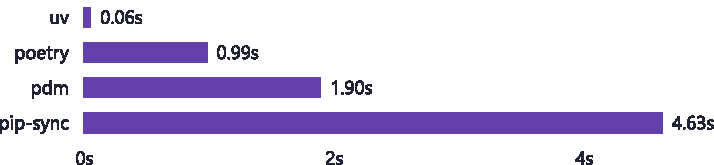
\includegraphics[width=0.7\textwidth]{graphics/speed.pdf}
    \src{docs.astral.sh/uv}
  \end{center}
\end{frame}

\begin{frame}[fragile]{How Do I Create a Package?}
  \begin{center}
    \huge\textcolor{ccyan!90!cblack}{\textbf{There is not \enquote{just one way} to create packages, but\dots}}
  \end{center}
  \vspace{1em}
  \begin{itemize}
    \setlength{\itemsep}{1em}
    \item Modern packaging uses a scaffolding called \texttt{pyproject.toml} with three important sections:
    \begin{description}[labelwidth=\widthof{\texttt{[build-system]}}]
      \item [\mintinline{toml}{[build-system]}] Allows you to describe what build backend to use.
      \item [\mintinline{toml}{[project]}] Sets up metadata for the package, such as the name or version.
      \item [\mintinline{toml}{[tool]}] A section for tool configuration.
    \end{description}
    \item An easy way to set up that scaffolding: \href{https://hatch.pypa.io/latest/}{{\footnotesize{\faExternalLink*}}\,\texttt{hatch}}
      \begin{minted}{shell-session}
        $ uv pip install hatch
        $ mamba install hatch
      \end{minted}
  \end{itemize}
\end{frame}

\begin{splitframe}[fragile]{How Do I Create a Package?}{Output}
  \begin{columns}[t,onlytextwidth]
    \begin{column}{0.58\textwidth}
      \begin{itemize}
        \item Use \textcolor{cpink}{\texttt{hatch}}'s CLI tool to quickstart creating a package:
          \begin{minted}{shell-session}
            $ hatch new my_package
          \end{minted}
      \end{itemize}
    \end{column}
    \hfill
    \begin{column}{0.38\textwidth}
      \begin{minted}{toml}
        my_package
        ├── src
        │   └── my_package
        │       ├── __about__.py
        │       └── __init__.py
        ├── tests
        │   └── __init__.py
        ├── LICENSE.txt
        ├── README.md
        └── pyproject.toml
      \end{minted}
    \end{column}
  \end{columns}
  \vspace{1em}
  \begin{columns}[t,onlytextwidth]
    \begin{column}{0.58\textwidth}
      \begin{itemize}
        \setlength{\itemsep}{1em}
        \item Let's see what this created:
          \begin{minted}{shell-session}
            $ head my_package/pyproject.toml
          \end{minted}
        \item You can also upgrade an existing project to use \texttt{hatch}:
          \begin{minted}{shell-session}
            $ hatch new --init
          \end{minted}
        \item Have a look at the \href{https://packaging.python.org/en/latest/guides/writing-pyproject-toml/}{{\footnotesize{\faExternalLink*}}\,Writing your \texttt{pyproject.toml}}
          guide to learn how to customise the \texttt{pyproject.toml} file
      \end{itemize}
    \end{column}
    \begin{column}{0.38\textwidth}
      \begin{minted}{toml}
        [build-system]
        requires = ["hatchling"]
        build-backend = "hatchling.build"

        [project]
        name = "my_package"
        dynamic = ["version"]
        description = ''
        readme = "README.md"
        requires-python = ">=3.8"
      \end{minted}
    \end{column}
  \end{columns}
\end{splitframe}

\begin{splitframe}[fragile]{Dependencies}{Example}
  \begin{columns}[t,onlytextwidth]
    \begin{column}{0.58\textwidth}
      \begin{itemize}
        \setlength{\itemsep}{1em}
        \item Dependencies for your project are defined with the \texttt{dependencies}
          key inside the \texttt{[project]} section
        \item You can set \href{https://packaging.python.org/en/latest/specifications/dependency-specifiers/}{{\footnotesize{\faExternalLink*}}\,dependency specifiers}
          (aka constraints) such as versions
      \end{itemize}
    \end{column}
    \hfill
    \begin{column}{0.38\textwidth}
      \begin{minted}{toml}
        [project]
        dependencies = [
          "numpy",
          "astropy<=6.1.0",
          "tomli;python_version<'3.11'",
        ]
      \end{minted}
    \end{column}
  \end{columns}
  \vspace{1em}
  \begin{columns}[t,onlytextwidth]
    \begin{column}{0.58\textwidth}
      \begin{itemize}
        \setlength{\itemsep}{1em}
        \item Define your optional dependencies in the \texttt{[project.optional-dependencies]} section
          and group them
        \item Install optional dependencies using
          \begin{minted}{shell-session}
            $ uv pip install my_package[plot]
          \end{minted}
      \end{itemize}
    \end{column}
    \hfill
    \begin{column}{0.38\textwidth}
      \begin{minted}{toml}
        [project.optional-dependencies]
        plot = ["matplotlib"]
      \end{minted}
    \end{column}
  \end{columns}
  \vspace{1em}
  \begin{columns}[t,onlytextwidth]
    \begin{column}{0.58\textwidth}
      \begin{itemize}
        \setlength{\itemsep}{1em}
        \item Fairly new (accepted \texttt{2024-10-10}): \href{https://peps.python.org/pep-0735/}{{\footnotesize{\faExternalLink*}}\,\texttt{PEP 735}} Dependency Groups
        \item Optional dependencies that are \emph{not} installed when a \emph{user} installs the package, \eg, via PyPI
        \item Install the groups from within your source repo:
          \begin{minted}{shell-session}
            $ uv pip install --group dev
          \end{minted}
      \end{itemize}
    \end{column}
    \hfill
    \begin{column}{0.38\textwidth}
      \begin{minted}{toml}
        [dependency-groups]
        tests = ["pytest", "pytest-cov"]
        docs = ["sphinx"]
        dev = [
          "jupyter",
          "pre-commit",
          {include-group = "tests"},
          {include-group = "docs"},
        ]
      \end{minted}
    \end{column}
  \end{columns}
\end{splitframe}

\begin{splitframe}[fragile]{CLI Scripts}{Example}
  \begin{columns}[t,onlytextwidth]
    \begin{column}{0.58\textwidth}
      \begin{itemize}
        \setlength{\itemsep}{1em}
        \item We can expose scripts in our package using the \texttt{pyproject.toml}
          \texttt{[project.scripts]} section
        \item Similarly: Entry points, that allow the creation of plugins, and cross-platform
          compatibility
          \begin{itemize}
            \item See \href{https://setuptools.pypa.io/en/latest/userguide/entry_point.html}{{\footnotesize{\faExternalLink*}}\,Entry Points}
          \end{itemize}
      \end{itemize}
    \end{column}
    \hfill
    \begin{column}{0.38\textwidth}
      \begin{minted}{toml}
        src/my_package/cli.py:
      \end{minted}
      \vspace{0.25em}
      \begin{minted}{python}
        def print_message():
            print("Hello World!")
            raise SystemExit(1)
      \end{minted}
      \vspace{1em}
      \begin{minted}{toml}
        pyproject.toml:
      \end{minted}
      \vspace{0.25em}
      \begin{minted}{toml}
        [project.scripts]
        hello-world = "my_package.cli:print_message"
      \end{minted}
      \vspace{1em}
      \begin{center}
        \huge\textcolor{cpink}{\texttt{\textbf{Result}}}
      \end{center}
      \begin{minted}[escapeinside=||]{toml}
        |\textbf{\textcolor{cpink}{\$}}| hello-world
        Hello World!
      \end{minted}
    \end{column}
  \end{columns}
\end{splitframe}


\secslide{Code Quality}

\secslide{Testing}

\begin{frame}{When Do We Need Tests?}
  \begin{center}
    \huge\textcolor{ccyan!90!cblack}{Imagine the following\dots}
  \end{center}
  \begin{itemize}
    \item You have written a package with a lot of code, \eg, multiple scripts
    \item You found a bug somewhere in your code
    \item You have not thought of possible edge cases during development
  \end{itemize}
  \vspace{1em}
  \begin{center}
    \huge\textcolor{cpink!90!cblack}{\to{} You will need to investigate your codebase for
    causes of the bug and the same bug may appear some time later}
  \end{center}
\end{frame}

\begin{frame}{Solution}
  \begin{center}
    \huge\textcolor{ccyan!90!cblack}{Write persistent tests \textbf{during development}!}\\
    \uncover<2>{\huge\textcolor{ccyan!90!cblack}{(And \textbf{automate} them \to{} see CI)}}
  \end{center}
\end{frame}


